\chapter{基于深度学习的缺陷检测}


本章将详细介绍如何将法线图应用到深度学习中,对零件进行缺陷检测。
首先我们会介绍卷积神经网络中的基本结构,
包括卷积层、激活函数、池化层、全连接层等,
接着介绍本文使用的神经网络模型的网络结构,
最后介绍如何对模型进行训练和测试,并给出实验结果和分析。

\section{基础结构}

本文使用卷积神经网络($Convolutional~Neural~Networks,\mbox{简称}~CNN$)结构进行缺陷检测。
卷积神经网络是一种层次模型,
它的输入是一张图像,
接着通过卷积($convolution$)操作、
池化\cite{chechik1998synaptic}($pooling$)操作和非线性激活函数($non-linear~activation~function$)映射等一系列操作的堆叠,
逐渐从原始图像提取出高维特征,
最后通过全连接层和输出层连接,
将目标任务(分类、回归等)形式化为目标函数,
并使用损失函数($loss~function$)
计算预测值和真实值之间的损失($loss$),
使用反向传播算法\cite{周志华2016机器学习}($back-propagation~algorithm$)将损失从后向前传播,更新参数,
如此反复直到模型收敛。

好的卷积神经网络模型得益于良好的网络结构设计,
而一个复杂精妙的网络结构往往由诸多基本结构组成,
本节首先介绍构成神经网络的一些基本结构,
这些结构将在接下来的网络结构以及实验等部分用到,
接着介绍网络模型的损失函数和优化方法。

\subsection{卷积层}

卷积是卷积神经网络中的基础操作。所谓卷积,就是使用一个固定大小的卷积核,通过滑动窗口的形式和图像对应区域做內积(逐个元素相乘再求和)操作,此时卷积核为一个固定大小的矩阵,这些矩阵的值即为该卷积核的权值。一般我们使用正方形的卷积核,并且其大小取奇数,常用的有$1\times 1$、$3\times 3$、$5\times 5$的卷积核,卷积核的大小即对应了滑动窗口的大小。
每完成一次卷积操作,卷积核移动一个位置,移动的大小记为卷积步长($stride$)。
因为图像是二维的,为了卷积整幅图像,需要卷积核向两个方向移动,因此卷积步长也是二维的,一般取$1\times 1$。

不难看出,卷积是一种局部操作,通过一定大小的卷积核作用于图像的局部区域,从而得到图像的局部信息,通过层层卷积,高层的卷积核可以扫过的信息会覆盖原始图片的更大区域,提取图像更高层的信息。需要注意的是,图片的底层特征往往与其在图片中的位置无关,因此我们在对图像做一次卷积时使用权值相同的卷积核,这被称为“权值共享”。权值共享大大减少了卷积层的参数,起到了防止过拟合的作用。

\subsection{激活函数}

激活函数层又称为非线性映射层,其引入正是为了增加整个网络的表达能力。如果没有激活函数层,那么整个网络仍可以看作是若干线性操作的堆叠,只能起到线性映射的作用。直观的看,激活函数模拟了神经元的特点:接收一组输入信号并产生输出。
激活函数的输入往往是卷积层卷积之后得到的值,因此通常激活函数层紧跟着卷积层,被合并为一层。

从定义来看,几乎所有的连续可导函数都可以作为激活函数,但是目前常见的多是分段性和具有指数形状的非线性函数,
本小节将介绍几种最基础的激活函数,
包括$Sigmoid$\cite{魏秀参解析卷积神经网络}函数、$Tanh$\cite{魏秀参解析卷积神经网络}函数和$ReLU$\cite{魏秀参解析卷积神经网络}函数。

\subsubsection{$Sigmoid$ 函数}

$Sigmoid$是使用范围最广的一类激活函数,
它是具有指数函数形状的激活函数。该函数的定义如公式\eqref{eq:sigmoid}所示。
\begin{equation}
\centering
f(x)=\frac{1}{1+e^{-x}}
\label{eq:sigmoid}
\end{equation}
其函数如图\ref{fig:Sigmoid}所示,从图中可以明显看出,经过$Sigmoid$型函数作用后,输出响应值的值域被压缩到$(0,1)$之间。
$Sigmoid$ 有其有利的一面,它在物理意义上最为接近生物神经元,并且$(0,1)$的输出范围可以理解为一个概率分布。
但是不难看出,
对于大于5(或小于-5)的值,无论多大(或多小)都会被压缩为1(或0),此部分的梯度会接近0,
从而导致在误差反向传播过程中该区域的误差很难传播,进而导致模型无法收敛,这一现象被称为“梯度消失”。
梯度消失可以被其它优化方法缓解,如Batch Normalization\cite{ioffe2015batch}。
\begin{figure}[htbp]
\centering
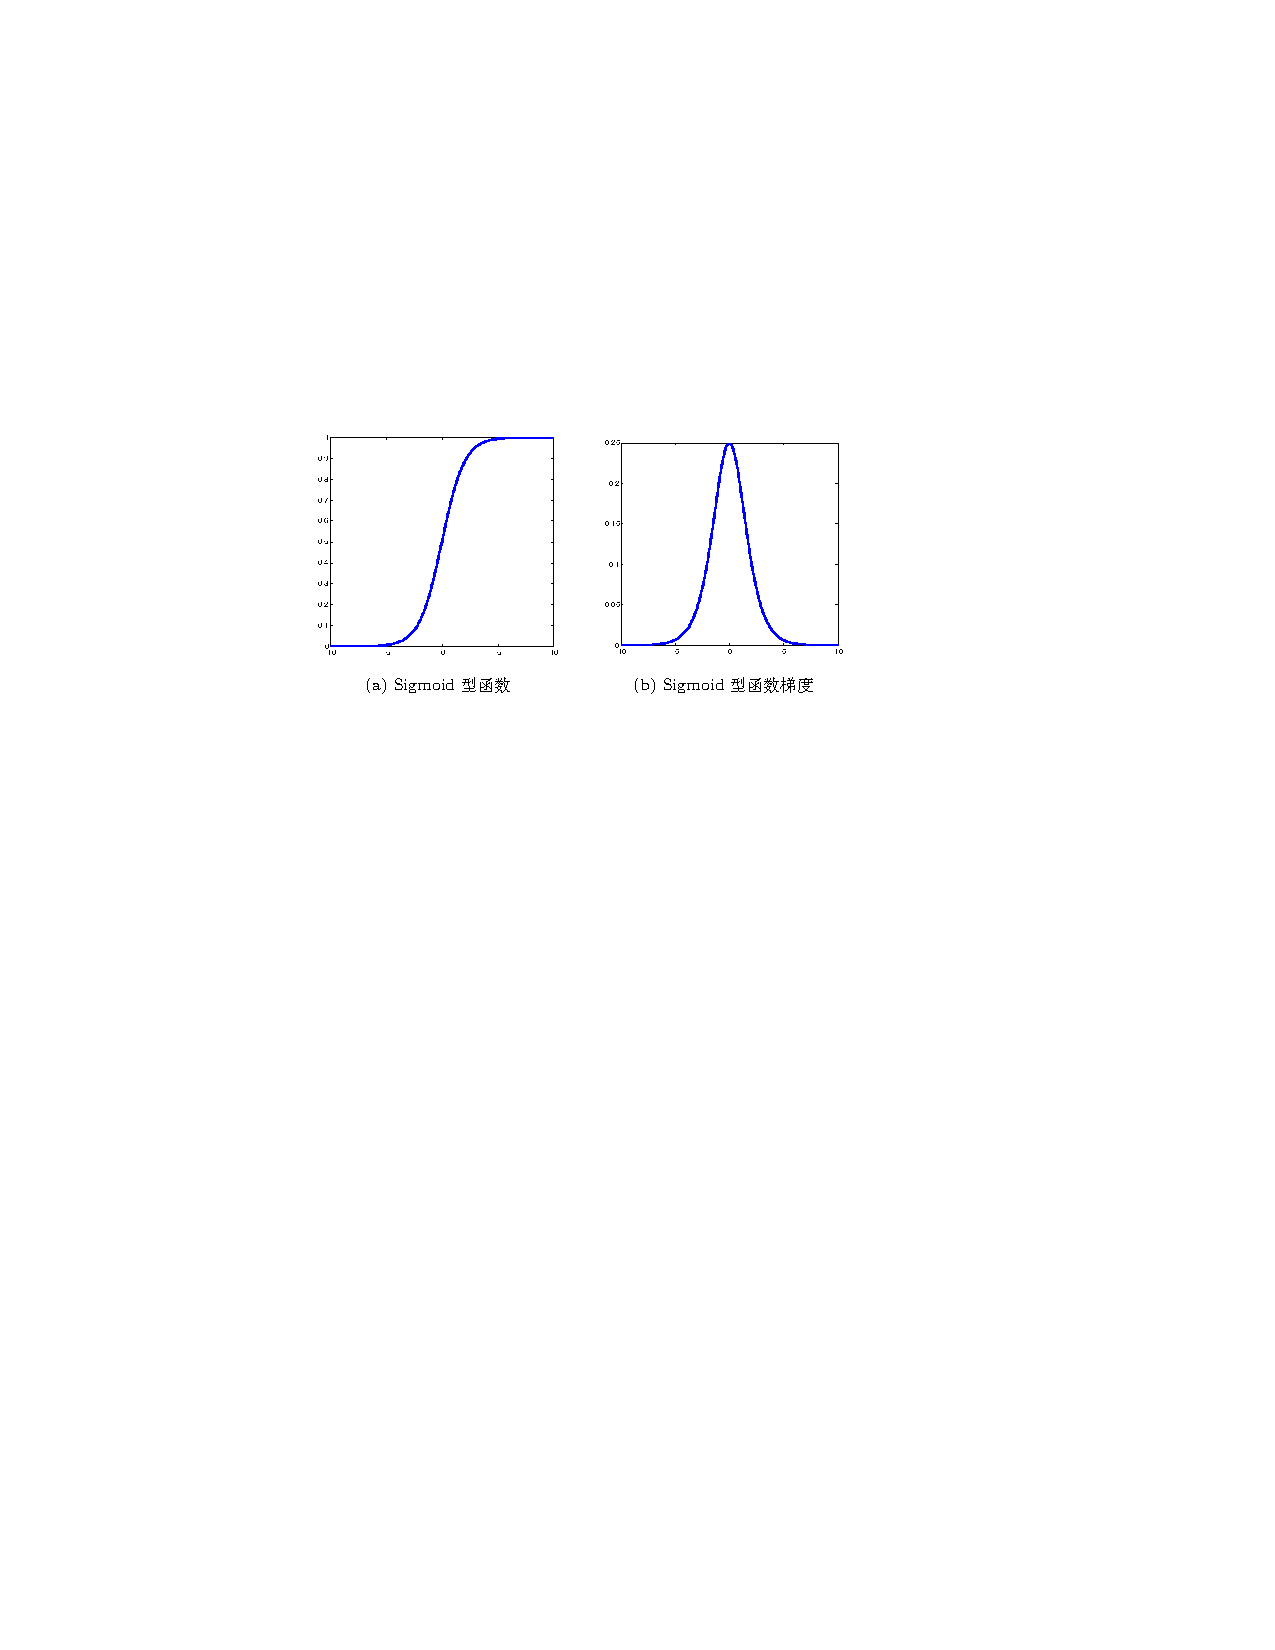
\includegraphics[width=0.7\linewidth]{figures/sigmoid.pdf} 
\caption{$Sigmoid$激活函数和其梯度示意图}
\label{fig:Sigmoid}
\end{figure} 

\subsubsection{$Tanh$ 函数}

$Tanh$激活函数又被称为双正切函数,
其形状与$Sigmoid$函数类似,都能将输出压缩到$(0,1)$,
但是该函数输出的均值比$Sigmoid$函数更接近0,在训练时收敛速度更快。
$Tanh$函数形式如公式\eqref{eq:tanh}所示。
\begin{equation}
Tanh⁡(x)=\frac{1-e^{-2x}}{1+e^{-2x}}
\label{eq:tanh}
\end{equation}
$Tanh$函数在$x$比较大或者比较小的时候仍会出现梯度消失的现象。


\subsubsection{$ReLU$ 函数}

$ReLU$\cite{nair2010rectified}是由Nair和Hinton在2010年提出的,
现已成为深度学习中最常用的激活函数之一。$ReLU$函数实际上是一个分段函数,其函数形式如公式\eqref{eq:relu}所示。
\begin{equation}
\centering
ReLU(x)=\max\{0,x\}
\label{eq:relu}
\end{equation}
与前两个激活函数相比,$ReLU$函数的梯度在$x\geq 0$时为1,反之为0,如图\ref{fig:relu}所示,
在$x\geq 0$的部分,该函数完全消除了梯度消失的情况,并且$ReLU$的计算复杂度更低,
在实际应用中能够更快的收敛。
$ReLU$的主要缺陷是在$x<0$时,
梯度为0,函数对这部分的卷积结果无法响应,
因此输入一旦变为负值将再无法影响网络的训练。
这一缺陷可以通过$Parametric~Rectified~Linear~Unit~(PReLU)$\cite{he2015delving}来改善。
\begin{figure}[htbp]
\centering
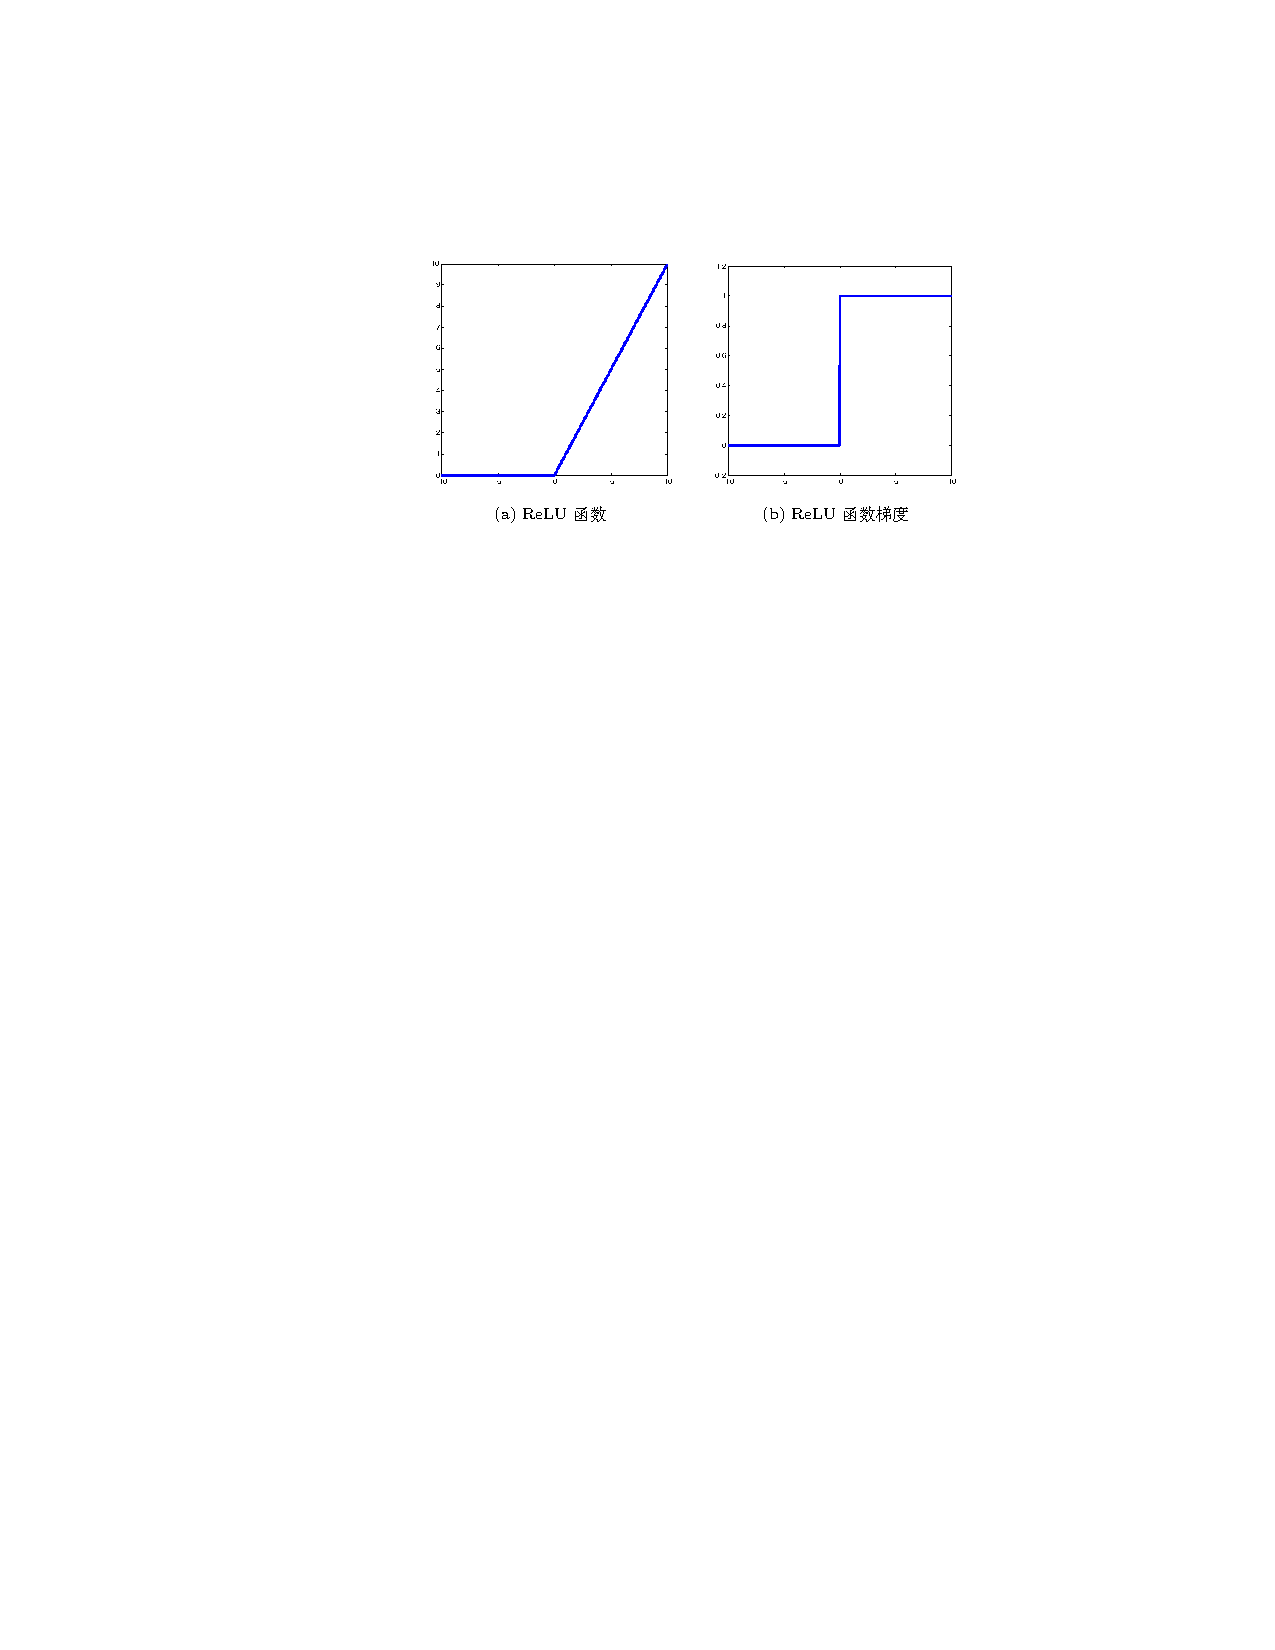
\includegraphics[width=0.7\linewidth]{figures/RELU.pdf}
\caption{$ReLU$激活函数和其梯度示意图}
\label{fig:relu}
\end{figure}

\subsection{池化层}

池化层一般采用平均池化($average-pooling$)或最大池化($max-pooling$)。
类似于卷积操作,池化层选择一个滑动窗口,取窗口中像素值最大值(最大池化层)或者平均值(平均池化层)作为池化操作的输出,可以对特征进行降维。从操作的角度来讲,池化层可以看做是一个用$p-$范数($p-norm$)作为非线性映射的“卷积”操作,当$p$趋近于正无穷时就是最大池化层。
与卷积层不同的是,池化层不需要设定参数,
使用时只需要指定池化层类型、池化操作的步长和核的大小即可。
从图像处理的角度来看,池化层可以被视为一种“降采样”,
一般卷积操作之后得到的特征可能会包含较多冗余信息,池化层的引入可以对特征进行降维和抽象,在一定程度上预防过拟合。
虽然池化层不是卷积神经网络中必须的,但是由于其良好的性质,往往会在卷积层之后使用池化层对特征降维。

\subsection{全连接层}

全连接层往往在整个卷积神经网络的最后一层或几层,起到“分类器”的作用。在这一层,每一个神经节点都会与上一层中的所有节点相连,因此全连接层往往含有较多参数。
如果说卷积层、激活函数和池化层是用来将原始数据映射到高维特征空间中的话,
那么全连接层就起到将特征映射到样本的标记空间中的作用。
实际应用中全连接层可以通过卷积操作实现,
当其前一层为全连接层时,可以通过$1\times 1$的卷积核实现,
当其前一层为卷积层时,可以通过与前一层特征维度大小一致的卷积核做全局卷积实现。

\subsection{损失函数}
\label{subseciont:sunshihanshu}

损失函数又被称为目标函数,被用来衡量预测值和真实样本标记之间的误差。在卷积神经网络中,
分类问题常用交叉熵损失函数作为目标函数,回归问题常用$l_2$损失函数作为目标函数。
\begin{equation}
\centering
L_{loss}=-\frac{1}{N}\sum_{i=1}^N(y_i\log{\hat{y_i}+(1-y_i)\log{(1-\hat{y_i})}})
\label{eq:lloss}
\end{equation}
本文将缺陷检测定义为一个二分类问题,
使用交叉熵损失函数$L_{loss}$作为目标函数,
其公式定义如\eqref{eq:lloss}所示,
其中N表示样本的数量,
$L_{loss}$表示整体损失。
$y_i$表示样本标签,当样本为缺陷样本时,
$y_i$值为1,
当样本为正常样本时,$y_i$值为0,
$\hat{y_i}$表示模型的输出,
它可以被看作该样本是缺陷样本的概率。
最终模型会输出样本为每个类的概率,
我们取概率最大的类作为最终预测的类。

\subsection{优化方法}

有了目标函数之后就可以针对目标函数优化网络参数,深度卷积神经网络通常采用随机梯度下降类的优化算法对模型参数优化。本节将介绍几种最常用的优化算法。

\subsubsection{随机梯度下降}

随机梯度下降算法($Stochastic~Gradient~Descent,\mbox{简称}~\mbox{SGD}$)是神经网络中最基础的优化算法,它根据误差的一阶梯度信息对参数调整,参数的更新策略可以用公式\eqref{eq:sgd}表示,
\begin{equation}
\centering
w=w-\eta \cdot dw
\label{eq:sgd}
\end{equation}
其中,$dw$表示误差对参数w的导数即梯度,它依赖于当前数据在目标函数上的误差,
我们利用误差的反向传播算法对其求解;
$\eta$表示学习速率,
是SGD算法中唯一的超参数,表示当前梯度值对网络参数更新的影响程度。
SGD算法收敛效果稳定,但是收敛速度较慢,并且,权值容易被困在鞍点,即$dw=0$的点,导致模型无法完全优化。SGD中学习率的设定也是一个问题,在选择学习率的时候,过大的学习率可能导致模型在训练阶段后期来回震荡,无法收敛,过小的学习率又会影响收敛速度。

\subsubsection{基于动量的随机梯度下降法}

受物理学研究的启发,
发展出了基于动量\cite{qian1999momentum}($Momentum$)的随机梯度下降算法,
该算法通过前几轮训练积累的“动量”信息辅助参数更新,更新策略用公式\eqref{eq:momentum}表示,
\begin{equation}
\begin{aligned}
\centering
v & =\mu \cdot v-\eta \cdot dw \\
w & =w+v
\end{aligned}
\label{eq:momentum}
\end{equation}
公式中,$\mu$为动量因子,表示动量对整体梯度更新的影响程度,
一般$\mu$取0.9;
$v$表示动量,在梯度方向相同的方向逐渐增大,
在梯度方向不同的方向逐渐变小;
$\eta$为学习率,
表示梯度$dw$对动量的影响。
基于动量的随机梯度下降法可以抑制SDG中会出现的震荡现象,
还可以帮助跳出鞍点,找到参数的更优解。

\subsubsection{RMSProp算法}

RMSProp($Root~Mean~Square~Prop$)算法\cite{hinton2012neural}可以针对学习率做动态的调整。这一算法的更新策略如\eqref{eq:rmsprop}所示,
\begin{equation}
\begin{aligned}
\centering
Sdw & =\beta \cdot Sdw-(1-\beta )dw^2 \\
w & =w- \alpha \frac{dw}{\sqrt{Sdw}+\varepsilon }
\end{aligned}
\label{eq:rmsprop}
\end{equation}
公式中加入了w的二阶导数对$Sdw$进行更新,在更新$w$的时候使用用$w$的梯度除以$Sdw$的平方根作为学习对象,
这使得对于不同的w可以有不同的学习率。其中$\varepsilon$只是为了防止分母变为0,本身对算法的意义不大,一般置为${10}^{-6}$,$\beta$为衰减因子,用于消除算法对全局学习率$\alpha$的依赖,
较大的$\beta$会促进网络更新,较小的$\beta$会抑制网络更新,一般可以取0.9,$\alpha$可以取1。

\subsubsection{Adam算法}

Adam\cite{kingma2014adam}算法用梯度的一阶矩估计和二阶矩估计动态调整每个参数的学习率,并且经过偏置校正后,每一次迭代学习率都有一个确定的范围,可以使得参数更新更加平稳。算法使用公式\eqref{eq:adam}调整参数$w$,调整时首先初始化$Vdw=0$,$Sdw=0$,
接着不断迭代更新参数,直到模型收敛。
\begin{equation}
\begin{aligned}
\centering
&Vdw  =\beta_1 \cdot Vdw-(1-\beta_1 )dw \\
&Sdw  =\beta_2 \cdot Sdw-(1-\beta_2 )dw^2 \\
&Vdw^{corrected}  =\frac{Vdw}{1-\beta_1^t}\\
&Sdw^{corrected}  =\frac{Sdw}{1-\beta_2^t}\\
&w  =w- \alpha \frac{Vdw^{corrected}}{\sqrt{Sdw^{corrected}}+\varepsilon }
\end{aligned}
\label{eq:adam}
\end{equation}
可以看出,Adam算法也需要指定参数,其中$\varepsilon$是为了防止分母为0,
使用${10}^{-6}$即可;$\beta_1$为第一矩参数,可以使用0.9;$\beta_2$为第二矩参数,
可以使用0.999。
该算法既考虑了动量又可以针对不同的参数调整学习率,常常具有较快的收敛速度和较好的效果。本文使用Adam算法对模型进行优化。

\section{网络模型}

本文使用VGG-11\cite{simonyan2014very}模型,
并对其进行了一定修改。
模型结构如图\ref{fig:VGG}所示,
图中用不同颜色的矩形标示出了不同种类的网络层。
第一层为输入层,输入图片的大小为$224\times224\times3$;
黑色矩形表示卷积层,
卷积核大小为$3\times3$,
步长为2。
论文中VGG11的卷积层后面紧跟$ReLU$激活层,
本文在卷积层之后、$ReLU$层之前加入了批归一化($Batch~Normalization$)层,
批归一化层由Sergey loffe和Christian Szegedy等人提出,
可以将数据归一化至均值为0、方差为1的分布。
这种方法有两个好处:首先它把输入的均值、方差规范化,保证了每一层的输入分布不发生改变,能够加快模型收敛;
其次它能起到轻微正则化的作用,预防过拟合。
红色矩形表示最大池化层,池化窗口大小为$2\times2$,步长为2。
浅蓝色矩形表示全连接层和紧随其后的$ReLU$激活层。
深蓝色矩形表示全连接层。
褐色矩形表示$Softmax$层,用于分类。

\begin{figure}[htbp]
\centering
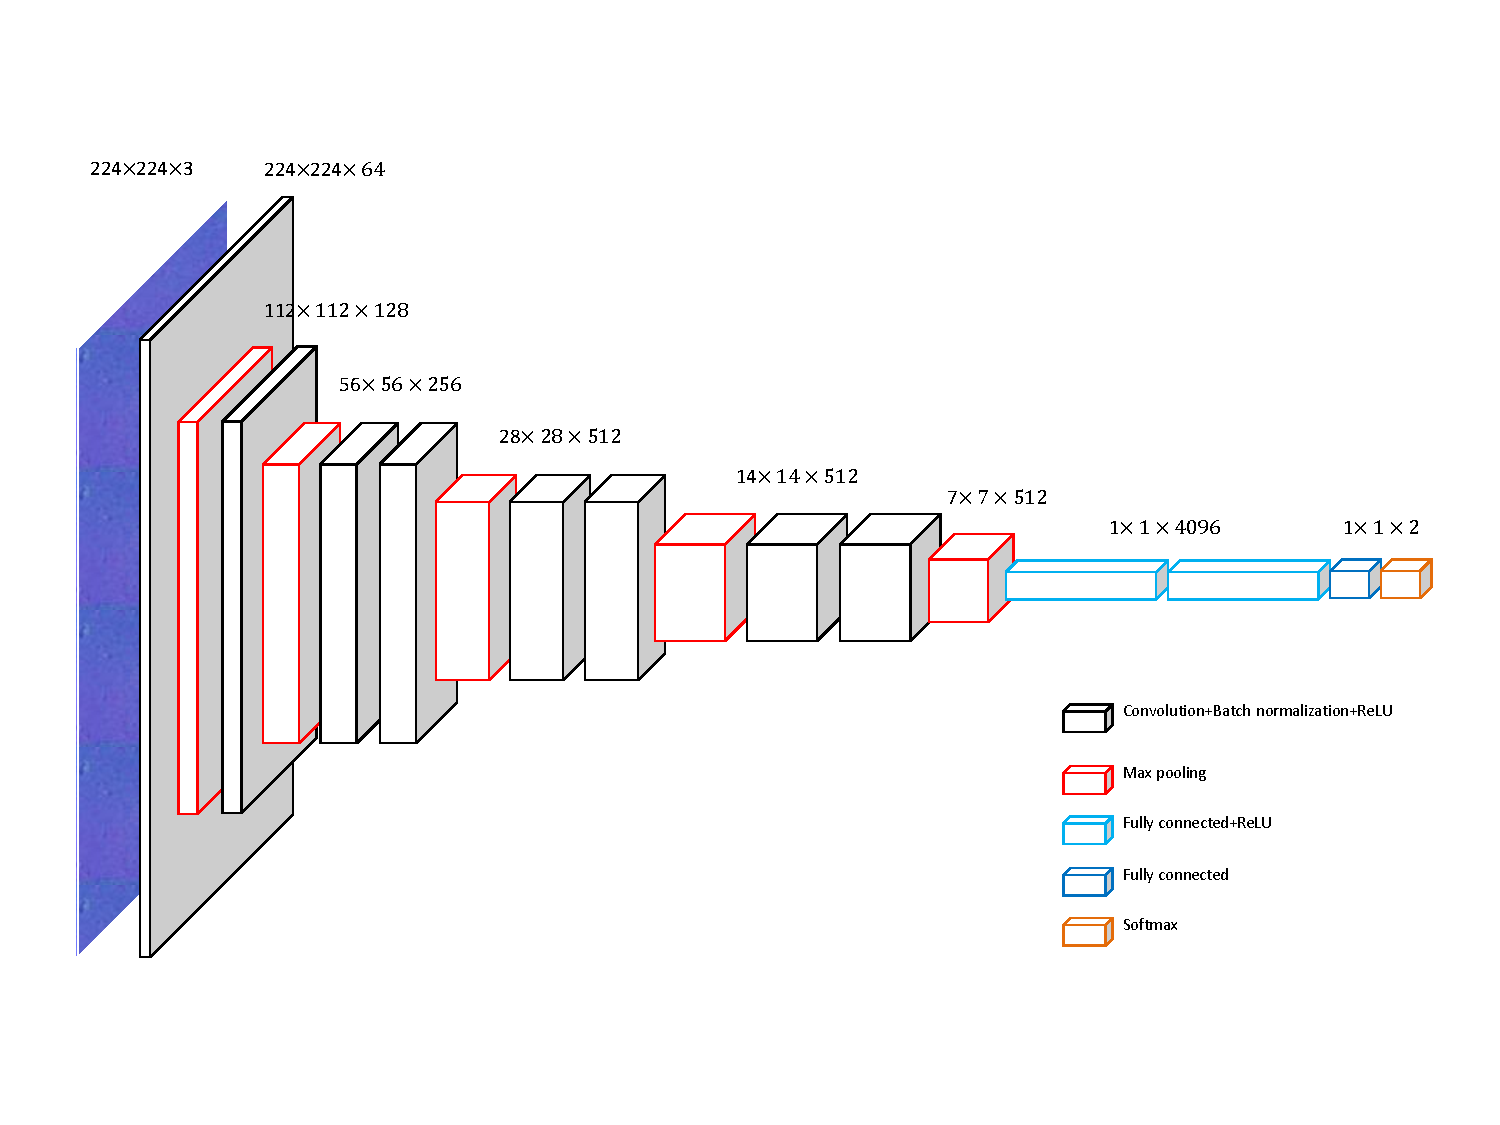
\includegraphics[width=1.0\linewidth]{figures/VGG.pdf}
\caption{VG-11模型结构示意图}
\label{fig:VGG}
\end{figure}

在训练阶段,我们使用$Dropout$方法来预防过拟合。
$Dropout$在向前传播时对神经元以一定的概率随机失活,这种失活只是暂时的,
每一轮训练时,都会以固定的概率重新失活神经元。
本文中$Dropout$失活概率取0.5。


\section{数据预处理}

同基于传统方法的缺陷检测一样,在使用深度学习进行缺陷检测时,数据的预处理也是非常重要的一环。
本章中的数据预处理方法和第\ref{chapter:chuantongfangfa}章类似,
我们首先提取零件的主表面,
接着用数据增强的方法扩大数据规模。

在提取零件主表面阶段,我们使用的方法没有任何变化,此处不再赘述。
在数据增强阶段,我们同样首先对数据做分割,
接着使用镜像和旋转增加样本数量,
但是VGG-11的输入是$224\times 224$,
同\ref{subsubssection:chuantongfenge}节中描述的图像分割方法不同,
本节中滑动窗口的大小为$40\times 40$,
接着我们使用双三次插值法将其放大为$224\times 224$。


\section{实验结果与分析}

本节将展示使用本章算法进行缺陷检测得到的结果,并将其与传统算法进行对比。
本文实验环境系统为Ubuntu 16.04,
使用的
Torch版本为0.3.1,
TorchVision版本为0.1.9。
实验计算机CPU为12核 Inter(R) Core(TM) i7-5820k @ 3.30GHz,
GPU为Tesla K40c,显存大小为11439M。


在训练阶段阶段,
我们首先用\ref{subsection:jilianjianceqi}中提到的方法
将数据集划分为不同的子数据集,
对每个子数据集训练一个网络模型,
最后使用级联的方式将其组合成一个级联检测器。
在模型训练时,
首先初始化模型,
然后优化参数,
直到模型收敛。
初始化模型时,
我们使用在ImageNet上预训练好的参数初始化模型。
在优化参数时,
优化的目标函数为\ref{subseciont:sunshihanshu}节定义的损失函数,
我们采用批处理随机梯度下降(mini-batch SGD)的方式训练模型,
$mini-batch$的大小设置为48,
读入数据时随机打乱数据的顺序。
我们使用Adam算法优化模型参数。
Adam中的学习率初始设为0.001,
$\beta_1$设置为0.9,
$\beta_2$设置为0.999,
训练过程会记录loss,
根据loss的变化情况
不断调整超参数。

我们分别训练了VGG-11、VGG-13、VGG-16和VGG-19,
并使用TensorboardX可视化训练过程。
不同模型的训练过程如图\ref{fig:vggshoulian}所示。
\begin{figure}[htbp]
\centering
\begin{minipage}{0.8\linewidth}
\centerline{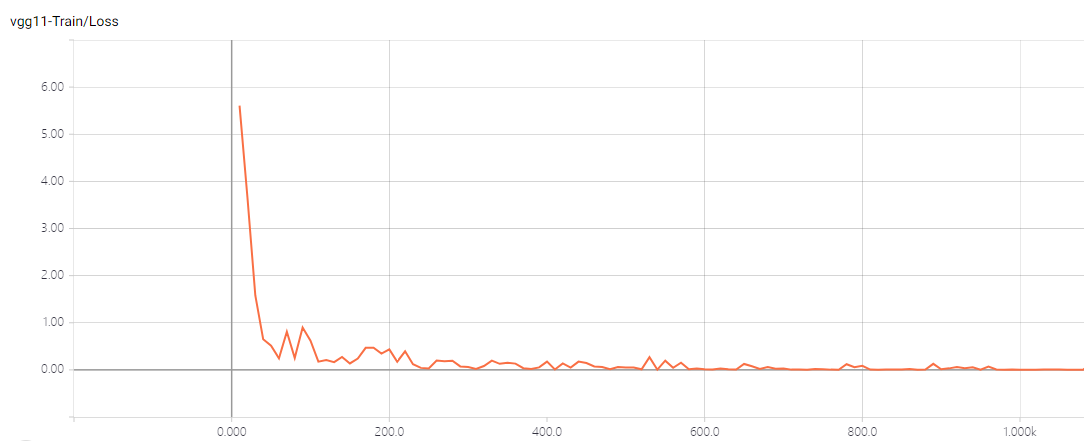
\includegraphics[width=1.0\linewidth]{figures/vgg11.png}}
\centerline{(a)}
\end{minipage}

\begin{minipage}{0.8\linewidth}
\centerline{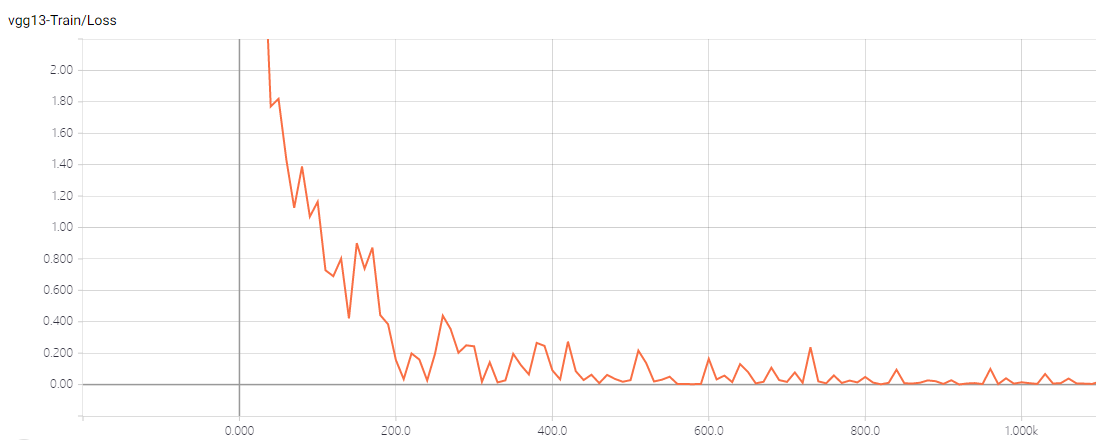
\includegraphics[width=1.0\linewidth]{figures/vgg13.png}}
\centerline{(b)}
\end{minipage}

\begin{minipage}{0.8\linewidth}
\centerline{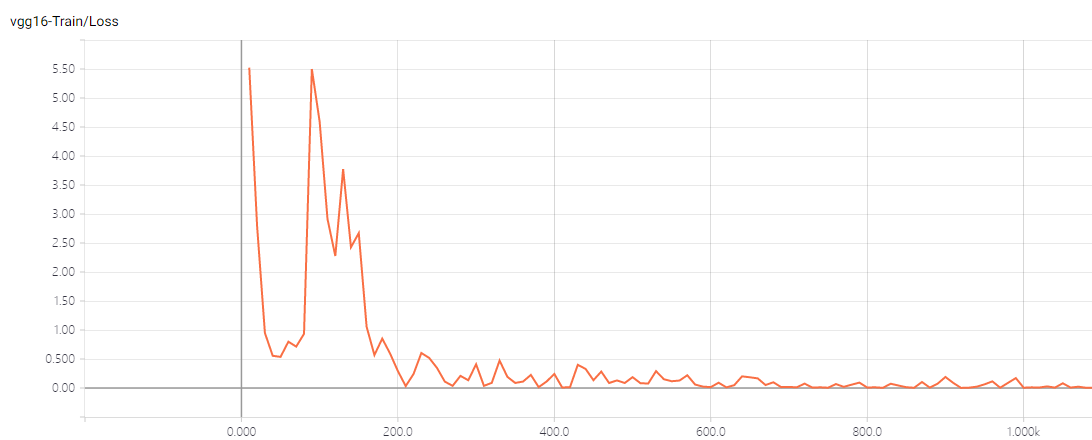
\includegraphics[width=1.0\linewidth]{figures/vgg16.png}}
\centerline{(c)}
\end{minipage}

\begin{minipage}{0.8\linewidth}
\centerline{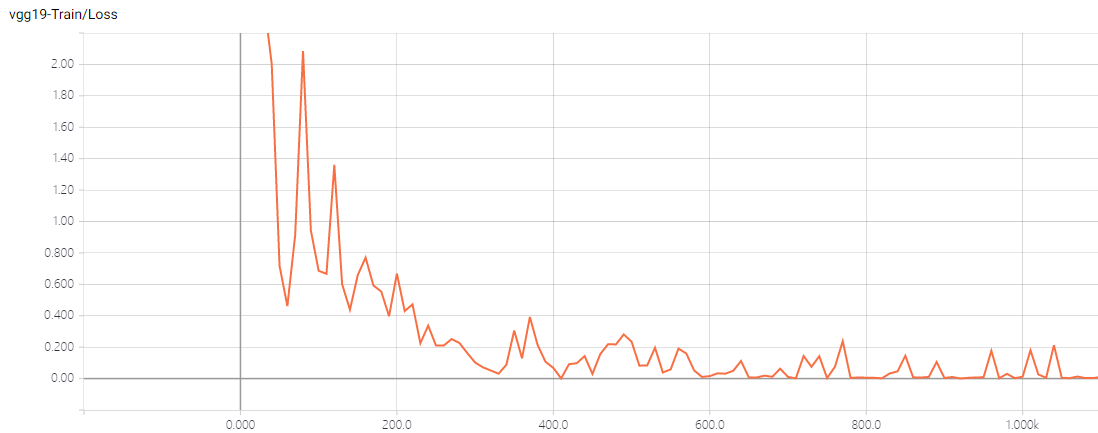
\includegraphics[width=1.0\linewidth]{figures/vgg19.png}}
\centerline{(d)}
\end{minipage}

\caption{VGG模型收敛示意图}
\label{fig:vggshoulian}
\end{figure}
图中
横轴表示训练轮数,
纵轴表示loss值,
我们每10轮统计一次loss值,
得到一个点,
将所有的点连起来得到折线。
图中$(a)$表示VGG-11的训练过程,
$(b)$表示VGG-13的训练过程,
$(c)$表示VGG-16的训练过程,
$(d)$表示VGG-19的训练过程。
不难发现,VGG-11收敛速度最快,
并且最稳定,
VGG-13和VGG-16收敛也比较快,
VGG-19的收敛则需要不断优化参数,
并且在模型的最后阶段容易出现震荡。
除此之外,
VGG-19有时会出现严重过拟合,
模型在训练集上效果极好,在测试集上却表现欠佳。
我们分析认为,造成这种现象的主要原因
是模型相对较复杂,需要大量数据训练,
而本文数据量不够充分。
这种过拟合的现象不仅出现在VGG-19中,
其它模型中也会有出现。

除此之外,每当我们用所有的数据训练一遍后,
我们都会使用测试集测试模型的表现,
记录测试集上效果最好的参数。
模型收敛后,
我们同样记录模型最终参数和其在测试集上的结果。
同基于传统方法的缺陷检测算法一样,
我们使用
召回率($REC$)、
查准率($PRE$)、
漏检率( $MDR$)、
误检率($FDR$)
作为模型评价标准。
评价标准中,
我们给予$REC$和$MDR$最高优先级,
即当两个模型进行比较时,
$REC$值越高,$MDR$值越低,
模型效果越好。
其次比较重要的评价指标是$PRE$,
最后是$FDR$。
\begin{table}[htbp]
\centering
\begin{tabular}{cccccp{38mm}}
\toprule
\textbf{模型类别} & \textbf{REC} & \textbf{PRE} & \textbf{MDR} & \textbf{FDR}\\
\midrule
\mbox{VGG-11} & 0.9735 & 0.8661 & 0.0265 & 0.0966\\
\mbox{VGG-13} & 0.9469 & 0.7643 & 0.0531 & 0.1875\\
\mbox{VGG-16} & 0.9646 & 0.8015 & 0.0354 & 0.1534\\
\mbox{VGG-19} & 0.9558 & 0.8120 & 0.0442 & 0.1420\\
\bottomrule
\end{tabular}
\caption{VGG模型最优结果表}
\label{tab:zuiyoujieguo}
\end{table}
\begin{table}[htbp]
\centering
\begin{tabular}{cccccp{38mm}}
\toprule
\textbf{模型类别} & \textbf{REC} & \textbf{PRE} & \textbf{MDR} & \textbf{FDR}\\
\midrule
\mbox{VGG-11} & 0.9643 & 0.7297 & 0.0356 & 0.1786\\
\mbox{VGG-13} & 0.9292 & 0.8468 & 0.0708 & 0.1080\\
\mbox{VGG-16} & 0.9548 & 0.8120 & 0.0452 & 0.1420\\
\mbox{VGG-19} & 0.9381 & 0.8281 & 0.0619 & 0.1250\\
\bottomrule
\end{tabular}
\caption{VGG模型最终结果表}
\label{tab:zuizhongjieguo}
\end{table}
表\ref{tab:zuiyoujieguo}中,展示了每个模型训练过程中得到的最优结果,
表\ref{tab:zuizhongjieguo}中展示了每个模型收敛后的结果。
从结果中可以看到,最终收敛后的参数往往在测试集上表现并非最好,
我们选择测试集上表现最好的模型参数作为最终参数。


考虑到过拟合问题,
我们将VGG-11模型进一步简化,
将模型中的最后两个卷积组各去掉一层,
其他网络结构保持不变,
将其记为VGG-9。
实验结果如表\ref{tab:jianhuajiegou}所示,
其中,VGG-9-best表示该模型在测试集上得到的最好结果,
VGG-9-final表示模型收敛后在测试集上的结果,
VGG-11-best和VGG-11-final则表示VGG-11的实验结果。
从实验结果来看,简化了模型结构并没有取得更好的结果,我们分析认为原因可能有两个:
首先,模型变得简单,描述能力下降;
其次由于我们调整了模型,
在使用ImageNet上预训练的参数初始化时,
只能初始化部分模型,
这使得模型中需要对参数的调整程度更大了。
\begin{table}[htbp]
\centering
\begin{tabular}{cccccp{38mm}}
\toprule
\textbf{模型类别} & \textbf{REC} & \textbf{PRE} & \textbf{MDR} & \textbf{FDR}\\
\midrule
\mbox{VGG-9-final} & 0.9027 & 0.7286 & 0.0973 & 0.2159\\
\mbox{VGG-9-best} & 0.9292 & 0.7143 & 0.0708 & 0.286\\
\mbox{VGG-11-final} & 0.9643 & 0.7297 & 0.0356 & 0.1786\\
\mbox{VGG-11-best} & 0.9735 & 0.8661 & 0.0265 & 0.0966\\
\bottomrule
\end{tabular}
\caption{VGG-9结果表}
\label{tab:jianhuajiegou}
\end{table}

综合上述实验结果,我们选择VGG-11作为我们的基础网络模型,
并将本章算法的实验结果和基于传统算法的实验结果进行对比。
如表\ref{tab:shenduxuexijieguo}所示,我们发现,本章算法的实验结果并不比使用HOG、Gredient和RGB联合特征训练出来的传统模型的结果好,我们认为最主要的原因有两点:首先在VGG-11中,输入数据的大小为$224\times 224$,虽然这是原始数据放大之后的结果,但由于缺陷目标往往较小,在这样的输入中,缺陷目标所占比例很小,而模型网络又比较深,使得缺陷区域的特征在最后的特征层中占比更小;其次,深度模型的训练往往需要大量数据,本文虽然使用数据增强增加了数据量,但仍不可避免出现一定的过拟合现象,导致模型泛化能力下降。
\begin{table}[htbp]
\centering
\begin{tabular}{cccccp{38mm}}
\toprule
\textbf{模型类别} & \textbf{REC} & \textbf{PRE} & \textbf{MDR} & \textbf{FDR}\\
\midrule
\mbox{HOG+Gredient+RGB} & 0.9915 & 0.8158 & 0.0085 & 0.0400\\
\mbox{VGG-11} & 0.9735 & 0.8661 & 0.0265 & 0.0966\\
\bottomrule
\end{tabular}
\caption{深度学习和传统方法检测结果表}
\label{tab:shenduxuexijieguo}
\end{table}
\begin{table}[htbp]
\centering
\begin{tabular}{cccccccp{38mm}}
\toprule
\mbox{模型类别} & \mbox{VGG-9} & \mbox{VGG-11} & \mbox{VGG-13} & \mbox{VGG-16} & \mbox{VGG-19}  \\
\mbox{检测速度} & 16ms & 23ms & 29ms & 34ms & 46ms  \\
\bottomrule
\end{tabular}
\caption{不同模型检测速度表}
\label{tab:jiancesudu}
\end{table}

基于我们的实验环境,不同模型的检测速度如表\ref{tab:jiancesudu}所示。
这里的检测速度是指将一个滑动窗口分类的速度,没有考虑加载模型的时间,
我们首先统计将所有测试集进行分类所用的时间,然后求其平均值作为模型的检测速度。
显然,随着模型深度的增加,模型的检测速度越来越慢。
